
\textbf{MathsResource.com}
\Large
\begin{itemize}
\item The continuous uniform distribution is very simple to understand and implement, and is commonly used in computer applications (e.g. computer simulation).
\item It is also known as the `Rectangle Distribution' for obvious reasons.
\end{itemize}
}
%---------------------------------------------------------------------------%
{
\textbf{MathsResource.com}
\Large
\begin{itemize}
\item We specify the word ``continuous" so as to distinguish it from it's discrete equivalent: the discrete uniform distribution.
\item Remark; the dice distribution is a discrete uniform distribution with lower and upper limits 1 and 6 respectively.
\end{itemize}
}

%-----------------------------------------------------%
{
\textbf{Uniform Distribution Parameters}
\Large

The continuous uniform distribution is characterized by the following parameters

\begin{itemize}
\item The lower limit $a$
\item The upper limit $b$
\item We denote a uniform random variable $X$ as $X \sim U(a,b)$
\end{itemize}

It is not possible to have an outcome that is lower than $a$ or larger than $b$.

\[ P(X < a) = P(X > b) = 0\]
}

%---------------------------------------------------------------------------%
{
\textbf{MathResource.com}
%{Continuous Uniform Distribution}
\vspace{-1cm}
\Large
A random variable X is called a continuous uniform random variable over the interval $(a,b)$ if it's probability density function is given by
\[ f_{X}(x) = { 1 \over b-a} \hspace{1cm} \mbox{ when } a \leq x \leq b \]\[\mbox{     (otherwise } f_X(x) = 0 ) \]
}
%---------------------------------------------------------------------------%
{
\textbf{MathResource.com}
%{Continuous Uniform Distribution}
\Large
The corresponding cumulative density function is
\[ F_x(x) = { x-a \over b-a} \hspace{1cm} \mbox{ when } a \leq x \leq b\]
}

%----------------------------------------------------------------------------------------------------%
{
%\textbf{MathResource.com}
%{Continuous Uniform Distribution}
\Large



\begin{center}
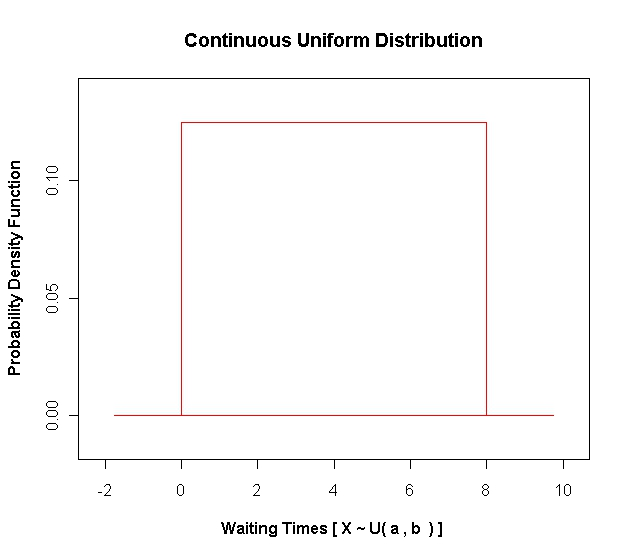
\includegraphics[scale=0.48]{6AUniform}

\end{center}
}



%------------------------------------------------------------------------%
{\textbf{Interval Probability}

\begin{itemize}
\item We wish to compute the probability of an outcome being within a range of values.
\item We shall call this lower bound of this range $L$ and the upper bound $ U$.
\item Necessarily $L$ and $U$ must be possible outcomes for the variable $X$.
\item The probability of $X$ being between $L$ and $U$ is denoted $P( L \leq X \leq U )$.

\begin{framed}
\[
P( L \leq X \leq U ) = { U - L \over b - a}
\]
\end{framed}
\item (This equation is based on a definite integral).
\end{itemize}
}

%---------------------------------------------------------------------------------------------------------%
{
\textbf{Uniform Distribution: Cumulative Distribution}
\Large
\begin{itemize}

\item For any value ``c" between the minimum value a and the maximum
value $b$, we can say
\item $P(X \geq c)$ \[P(X \geq c) = {b-c \over b-a}\]
here $b$ is the upper bound while $c$ is the lower bound
\item $P(X \leq c)$ \[P(X \leq c) = {c-a \over b-a}\]
here $c$ is the upper bound while $a$ is the lower bound.
\end{itemize}
}

%-----------------------------------------------------------------------------%
{
\textbf{Uniform Distribution: Mean and Variance}
\Large
\begin{itemize}
\item The Expected Value (in other words, the mean)  of the continuous uniform variable $X$ , with parameters $a$ and $b$ is
\[ \mathrm{E}(X) = {a+b \over 2}\]
\item The variance is computed as
\[ \mathrm{Var}(X) = {(b-a)^2 \over 12}\]
\end{itemize}
}

%---------------------------------------------------------------------------%
{
\textbf{Continuous Uniform Distribution}
A random variable X is called a continuous uniform random variable over the interval $(a,b)$ if it's probability density function is given by

\[ f_{X}(x)  =  { 1 \over b-a}   \hspace{2cm}  \mbox{ when } a \leq x \leq b\]

The corresponding cumulative density function is

\[ F_x(x) = { x-a \over b-a}   \hspace{2cm}  \mbox{ when } a \leq x \leq b\]

}






\end{document}

						
0	 < X <	0.16667	&	1	 \\ \hline	
0.16667	 < X <	0.33333	&	2	 \\ \hline	
0.33333	 < X <	0.50000	&	3	 \\ \hline	
0.50000	 < X <	0.66667	&	4	 \\ \hline	
0.66667	 < X <	0.83333	&	5	 \\ \hline	
0.83333	 < X <	1.00000	&	6	 \\ \hline	


%--------------------------------------------------------------------------------%

0.9041541					6	 \\ \hline
0.9305909					6	 \\ \hline
0.1866838					2	 \\ \hline
0.4378959					3	 \\ \hline
0.588299					4	 \\ \hline
0.1617157					1	 \\ \hline

 
